\documentclass[./../main.tex]{subfiles}
\graphicspath{{img/}}

\begin{document}
    \begin{exercise}
        Dibuja y explica el arreglo de imanes utilizado para enfocar o desenfocar haces de partículas.

        \begin{solution}
            Además de curvar los haces de partículas (dipolo magnético), también es necesario enfocarlos. Enfocar el haz permite que su altura y anchura se reduzcan para que se limite a la cámara de vacío del acelerador. Esto se logra mediante el uso de un arreglo específico de imanes, conocido como \textbf{cuadrupolo magnético}, o lentes magnéticos, que actúan de la misma manera que las lentes ópticas sobre un rayo de luz. El cuadrupolo consiste de cuatro polos magnéticos; el campo se desvanece en el centro y su magnitud aumenta conforme nos alejamos de él.

            \begin{figure}[htb]
                \centering
                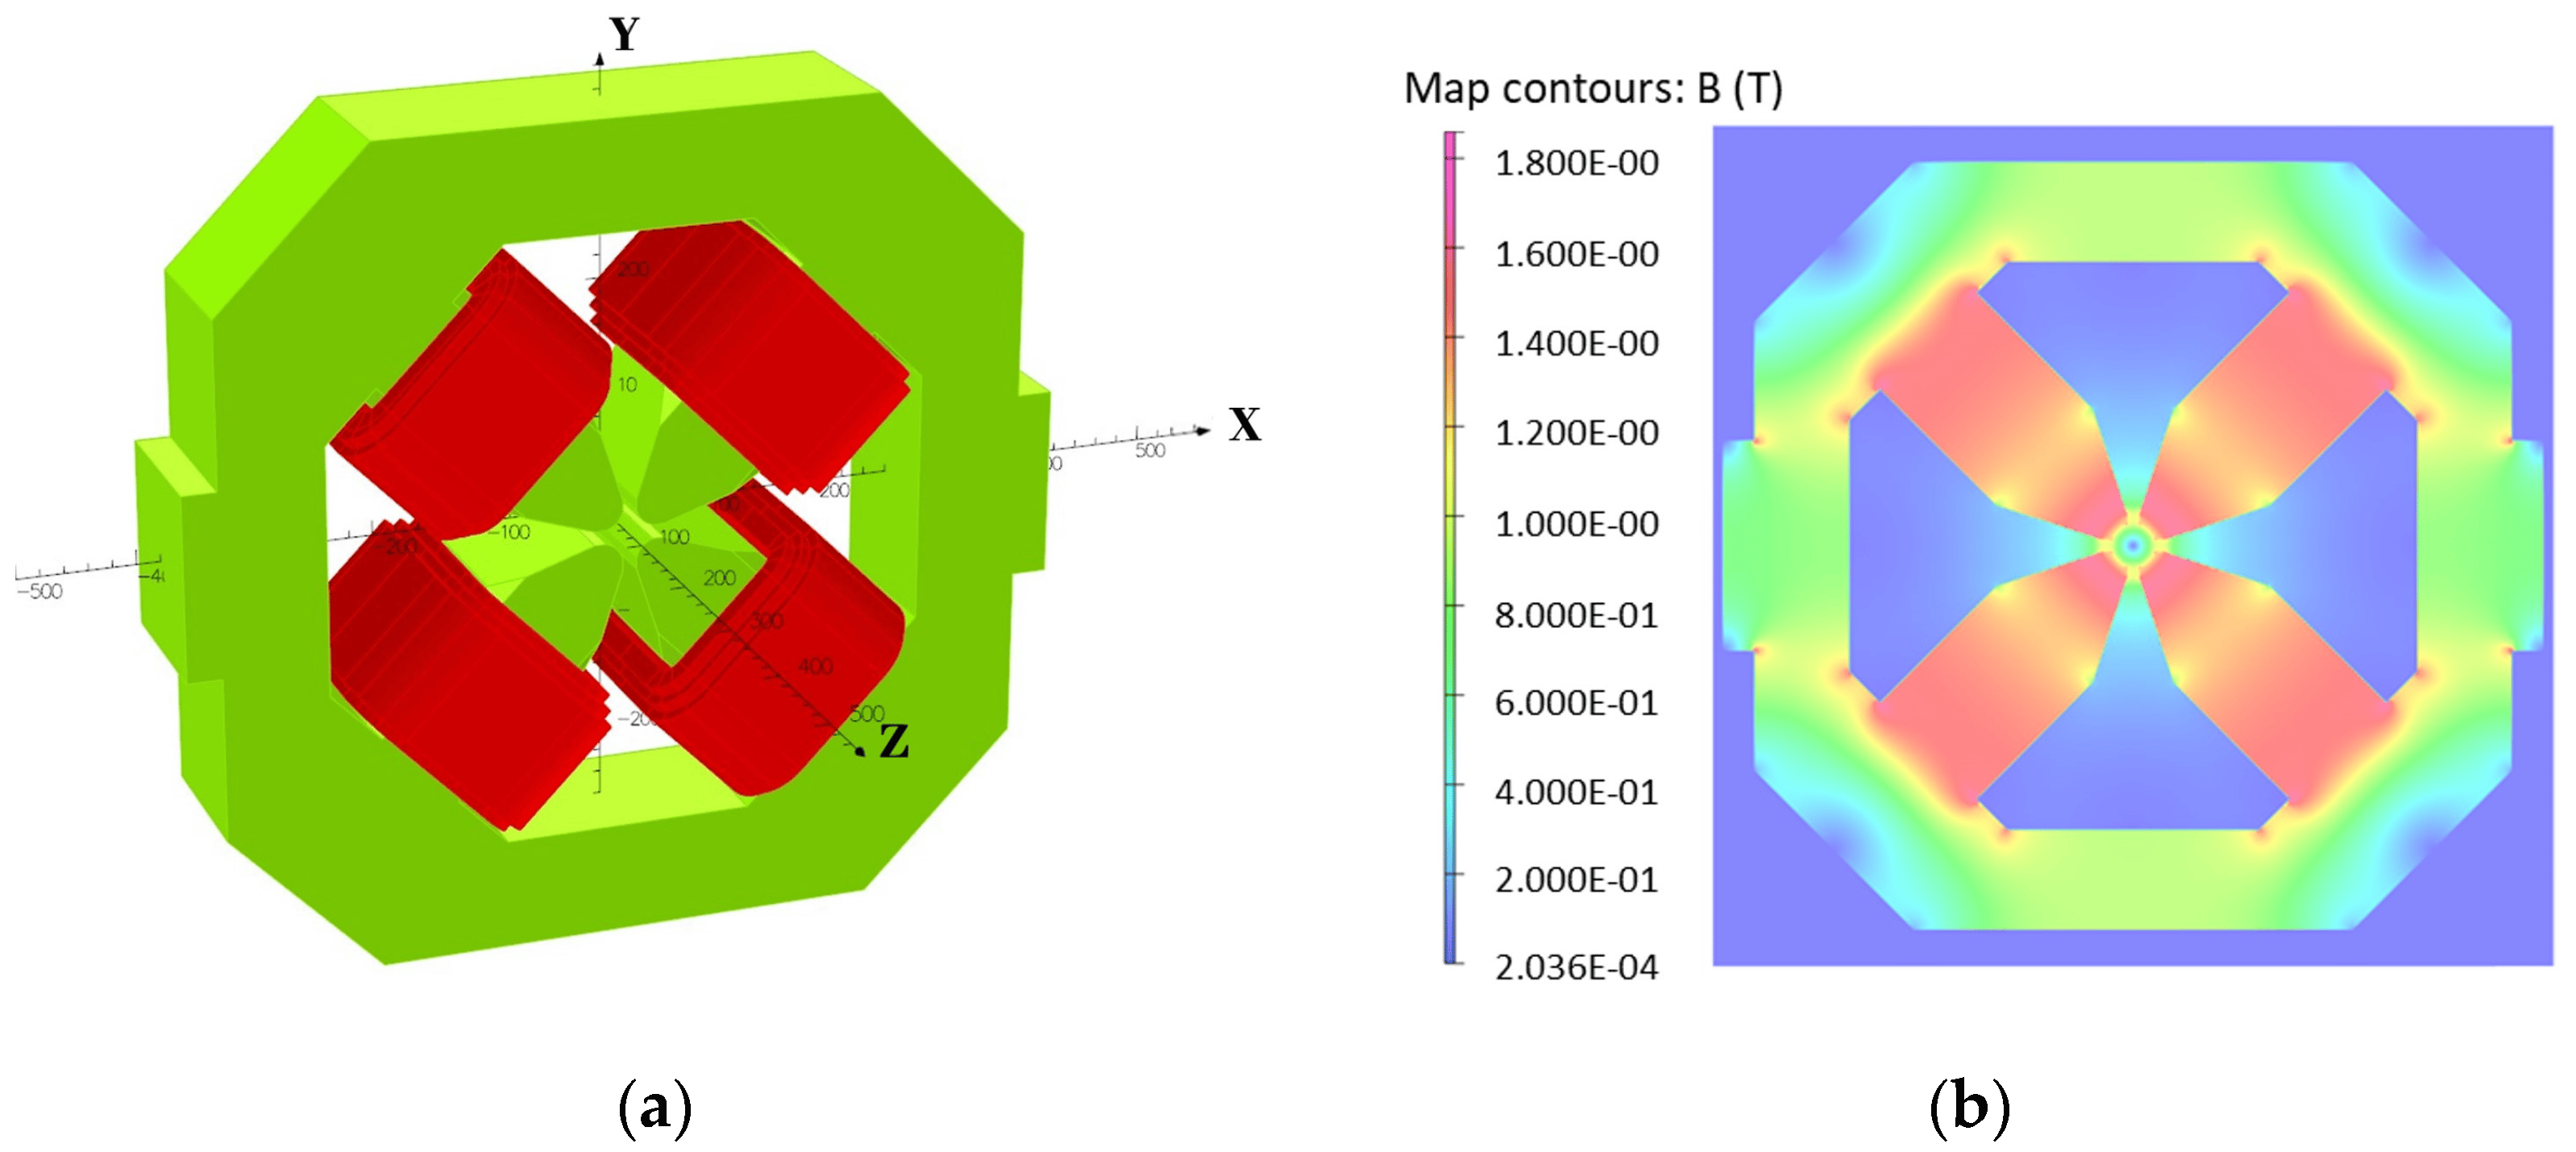
\includegraphics[scale=0.2, trim={0cm 7cm 57cm 0}, clip]{quadrupole}
                \caption{Diagrama de un cuadrupolo magnético. \parencite{prawanta2023development}}
                \label{fig:cuadrupolo}
            \end{figure}            

            El principio que rige este efecto, el de enfocar o desenfocar, se conoce como enfoque fuerte (o \emph{strong focusing}, por su nombre en inglés).

            Para explicar su funcionamiento imaginemos una partícula positivamente cargada (ver \cref{fig:quadrupole-principle}) que entra en la región a lo largo del eje del imán (\(x = y = 0\)). Para este caso, la superposición de las líneas de campo magnético es tal que sus efectos son nulos. Ahora supongamos que la partícula entra en dirección con \(x = 0\) (\(y \neq 0\)); para \(y\)'s positivas como negativas, conforme la partícula atraviesa el campo magnético esta se desvía al centro de la apertura del imán. Entre mayor sea el valor de \(\abs{y}\) de la partícula, mayor será el campo magnético y la desviación de la partícula; por lo que para cualquier partícula positivamente cargada que entre por esta región del campo del cuadropolo sufrirá un efecto de enfoque. 
            Para partículas que lleguen con dirección \(y = 0\) (\(x \neq 0\)), el efecto es el contrario, \idest el cuadrupolo desenfoca las partículas.

            \begin{figure}[htb]
                \centering
                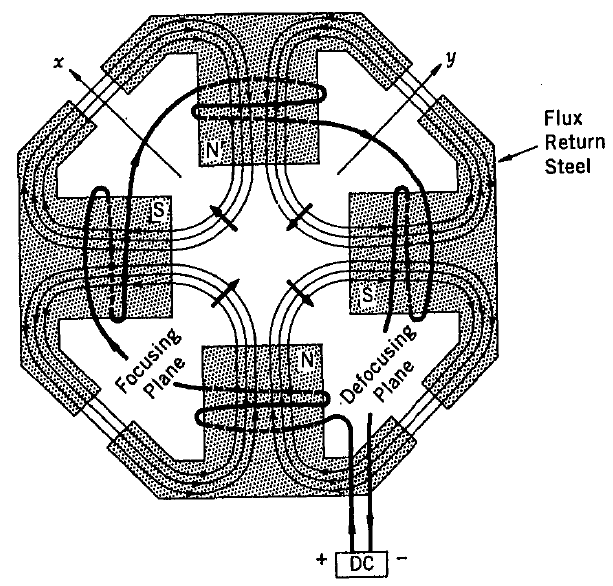
\includegraphics[scale = 0.8]{quadrupole-principle}
                \caption{Funcionamiento de un cuadrupolo magnético. \parencite{das2003introduction}}
                \label{fig:quadrupole-principle}
            \end{figure}

            Y puesto que queremos mantener control de la altura y anchura del haz debemos tener una secuencia de cuadrupolos que desenfoquen y enfoquen el haz, como se observa en la siguiente figura.

            \begin{figure}[htb]
                \centering
                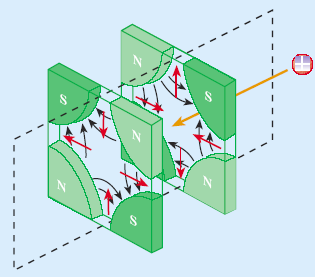
\includegraphics{quadrupole-array}
                \caption{Secuencia de cuadropolos magnéticos para enfocar y desenfocar el haz de partículas. \parencite{LHC2023}}
            \end{figure}
        \end{solution}
    \end{exercise}
\end{document}